\setcounter{chapter}{1}
\chapter{フーリエ解析入門}
%
波動や振動現象など,何らかの系の状態を表す関数が周期的に振る舞うものは
私たちの身の周りに溢れている.
例えば,私たちに近い分野でみると,
種々の分光学的測定で得られる時系列データ(信号)は周期関数(とみなせるもの)である.
それらは一見するとグチャグチャしていて,ただ漠然と眺めているだけでは新しい知見は得られない.
そうではなく,例えば,その信号の中にはどういった振動数の波がどの程度含まれているか,
などを取り出すことが出来れば,その現象の理解を深めることができる.
その要求に答える数学的手法がフーリエ (Fourier)解析である.
この例に限らず,フーリエ解析は極めて広い分野で使われる強力な手法であり,
前章で学んだ微分方程式を解く際にも有効である.
そこで,この章ではフーリエ解析について学んでいくことにする.
ただし,「フーリエ解析」という名前で1期分の講義があるくらいで,
フーリエ解析に関する諸事項を幅広くかつ厳格に述べるには圧倒的に時間が足りないので,
かなり初歩的な事項を紹介するに留めざるを得ないが,それでも応用範囲は広い.

%しかし,
%ここでは,近い将来皆さんが化学工学の分野で研究を進めていてフーリエ解析
%の知識が必要に
%
\section{フーリエ級数}
%
皆さんにとって馴染みのあるテイラー展開について考えてみよう.
テイラー展開とは,次式のように
関数$f(x)$をべき級数として展開する,というものであった.
\begin{align}
  f\left(x\right) &= f\left(a\right) + f^{\prime}\left(a\right)
 \left(x-a\right) + \dfrac{f^{\prime\prime}\left(a\right)}{2!}\left(x-a\right)^{2} + \cdots. 
\end{align}
%
上述のように,テイラー展開ではべき級数となるが,$x^{0},~x^{1},~x^2,~x^3,\cdots$以外にも,何らかの関数のセットで展開出来るのではないか
と考えることは,一般性を重んじる(ことが多い)数学の立場からすると自然なことである.実際,そのような関数のセットを系統立てた考えの元に
用意することは可能で\footnote{このあたりの話はとても面白いのだが,時間の都合上省略する.興味が出た人は直交関数やグラム-シュミットの直交化法といったキーワードで調べてみると良い.決して難しくはない.},
関数のセットの一つとして,三角関数(sin, cos)が挙げられる.
周期関数を展開する際に,三角関数を用いるのはもっともらしいように思える.実は周期関数を三角関数を用いて展開して得られるものをフーリエ級数と呼び,これから学んでいくことになる.

まずは,周期関数について整理しておく.
周期$L~(>0)$の関数$f(x)$とは,
\begin{align}
  f\left(x + L\right) = f\left(x\right), 
\end{align}
を満たす関数のことを指す.
また,もし$a\leq x \leq b$の範囲で定義されている関数の場合は,
それを周期$b-a$の周期関数と一部とみなして,全区間に拡張することができる.
%
\begin{figure}[htbp]
  %\includegraphics[width=1.0\linewidth]{figures/extend_function.eps} 
  \includegraphics[width=1.0\linewidth]{/Users/kasa/Dropbox/GitHub/lectures/osaka-u/2021/kaenI/chap02_fr/figures/extend_function.eps} 
\end{figure}
%
\subsection{三角関数に関する諸公式}
%
フーリエ解析で現れる式変形では,割と高い頻度で高校数学で学んだタイプの三角関数の定理や積分
が現れる.それをその都度証明していくのは大変なので,ここで公式としてまとめておく.
\begin{align}
 &\sin\left(\alpha \pm \beta\right) = \sin\alpha \cos \beta \pm \cos\alpha \sin\beta, \\
 &\cos\left(\alpha \pm \beta\right) = \cos\alpha \cos \beta \mp \sin\alpha \sin\beta, \\
 &\sin^{2} \alpha = \dfrac{1-\cos 2\alpha}{2}, \\
 &\cos^{2} \alpha = \dfrac{1+\cos 2\alpha}{2}, \\
 &\sin \alpha \cos \beta = \dfrac{1}{2}\left(\sin(\alpha+\beta)+\sin\left(\alpha -\beta\right)\right), \label{tri_formula_01} \\
 &\sin \alpha \sin \beta = \dfrac{1}{2}\left(\cos(\alpha-\beta) - \cos(\alpha+\beta)\right). \label{tri_formula_02} 
\end{align}

また,$m,~n$を自然数として次式が成り立つ.
\begin{align}
 &\int_{0}^{2\pi}dx\,\cos nx = 0,  \label{tri_intformula_01} \\
 &\int_{0}^{2\pi}dx\,\sin nx = 0,  \label{tri_intformula_02} \\
 &\int_{0}^{2\pi}dx\,\cos mx \cos nx = 0\, \quad (m\neq n) \label{tri_intformula_03} \\
 &\int_{0}^{2\pi}dx\,\cos^{2} nx = \pi, \label{tri_intformula_04} \\
 &\int_{0}^{2\pi}dx\,\cos mx \sin nx = 0, \label{tri_intformula_05} \\
 &\int_{0}^{2\pi}dx\,\sin mx \sin nx = 0, \quad (m\neq n) \label{tri_intformula_06} \\
 &\int_{0}^{2\pi}dx\,\sin^{2} nx = \pi. \label{tri_intformula_07}
\end{align}
ここでは積分区間を$0\leq x \leq 2\pi$にしているが,これを定数分だけずらした区間$a\leq x \leq a + 2\pi$で
あっても上式は成り立つ.
%
\subsection{複素フーリエ級数}
%
それでは実際に周期関数をフーリエ級数の形で表すことを考えてみよう.
まず大事なことは,周期$L$の関数$f\left(x\right)$を展開するために用いる
三角関数も周期$L$の関数でなければならない,ということである.
$\sin x$, $\cos x$は周期$2\pi$の関数であるから,これらを周期$L$にするためには引数をいじって,
\begin{align}
  \sin\left(\dfrac{2\pi n}{L}x\right),\quad \cos\left(\dfrac{2\pi n}{L}x\right),
\end{align}
とすれば良い.ただし,$n$は整数である.ここでは,オイラーの公式を用いて,sin関数とcos関数をまとめて,
\begin{align}
 \exp\left(i\dfrac{2\pi n}{L}x\right),
\end{align}
にしておいて,$f\left(x\right)$を次式のように展開してみる.
\begin{align}
 f\left(x\right) = \sum_{n=-\infty}^{\infty} c_{n} \exp\left(i\dfrac{2\pi n}{L}x\right). 
\end{align}
これを複素フーリエ級数と呼ぶ.
級数展開では,その展開係数$c_m$を求めることが重要となるが,実は前節でまとめた公式を使うとすぐ求められる.
両辺に$\exp(-i\frac{2\pi m}{L}x)$をかけて,区間$-L/2 \leq x \leq L/2$で積分すると
\footnote{周期関数の場合は周期1つ分を含んでいれば良い.今回は対称性を意識して$-L/2 \leq x \leq L/2$としている.},左辺は
\begin{align}
\int_{-L/2}^{L/2}dx\,f\left(x\right)\exp\left(-i\dfrac{2\pi m}{L}x\right),
\end{align}
である(特に式変形はしていない).左辺は,
\begin{align}
 &\sum_{n=-\infty}^{\infty}c_n\int_{-L/2}^{L/2}dx\,\exp\left(-\dfrac{2\pi}{L}\left(n-m\right)x\right) \notag \\
 &=\sum_{n=\infty}^{\infty}c_n\int_{-L/2}^{L/2}dx\,\left\{\cos\left(\dfrac{2\pi}{L}\left(n-m\right)x\right) 
   + i\sin\left(\dfrac{2\pi}{L}\left(n-m\right)x\right)\right\},
\end{align}
である.ここで,$(2\pi/L)x = X$と変数変換すると,$dx = (L/2\pi)dX$,また 
積分区間は$-\pi\leq X \leq \pi$となるので,
\begin{align}
  \dfrac{L}{2\pi}  \sum_{n=-\infty}^{\infty} c_n \int_{-\pi}^{\pi}dX\, \left\{\cos\left(\left(n-m\right)X\right) + i\sin\left(\left(n-m\right)X\right)\right\},
\end{align}
である.$n=m$のときは,
\begin{align}
 \dfrac{L}{2\pi}  c_m \int_{-\pi}^{\pi}dX\, \left\{\cos\left(\left(n-m\right)X\right) + i\sin\left(\left(n-m\right)X\right)\right\} = \dfrac{L}{2\pi}c_{m}\int_{-\pi}^{\pi}dX = Lc_{m},
\end{align}
となり,$n\neq m$のときは\Eq{tri_intformula_01}と\Eq{tri_intformula_02}から,
\begin{align}
 \dfrac{L}{2\pi}   c_n \int_{-\pi}^{\pi}dX\, \left\{\cos\left(\left(n-m\right)X\right) + i\sin\left(\left(n-m\right)X\right)\right\} = 0, 
\end{align}
となる.つまり,結局生き残るのは$n=m$の項だけとなり,
\begin{align}
  c_m = \dfrac{1}{L}\int_{-L/2}^{L/2}dx\,f\left(x\right)\exp\left(-i\dfrac{2\pi m}{L}x \right), 
\end{align}
を得る.これが複素フーリエ級数の展開係数の表式である.この展開係数のことをフーリエ係数と呼ぶ.
今後の便宜のため,式を以下にまとめておく.
\begin{align}
 & f\left(x\right) = \sum_{n=-\infty}^{\infty} c_{n} \exp\left(i\dfrac{2\pi n}{L}x\right), \label{complex_fourier}\\
 & c_n = \dfrac{1}{L}\int_{-L/2}^{L/2}dx\,f\left(x\right)\exp\left(-i\dfrac{2\pi n}{L}x \right). \label{complex_fourier_coef}
\end{align}
%
\subsection{実フーリエ級数}
%
複素フーリエ級数は,$\exp(i\frac{2\pi n}{L}x)$を展開に用いているが,
これを$\sin(\frac{2\pi n}{L}x)$と$\cos(\frac{2\pi n}{L}x)$で表してみよう.
\Eq{complex_fourier}の和を$n=0$, $n=-\infty\sim -1$, $n=1\sim \infty$に分けてみると,
\begin{align}
  f\left(x\right)
  &= c_{0} + \sum_{n=-\infty}^{-1}c_n \exp\left(i\dfrac{2\pi n }{L}x\right) 
    + \sum_{n=1}^{\infty} c_n \exp\left(i\dfrac{2\pi n }{L}x\right) \notag \\
  &= c_{0} + \sum_{n=1}^{\infty}c_{-n}\exp\left(-i\dfrac{2\pi n}{L}x\right) 
   + \sum_{n=1}^{\infty}c_{n} \exp\left(i\dfrac{2\pi n}{L}x\right) \notag \\
  &= c_{0} + \sum_{n=1}^{\infty}\left\{\left(c_n + c_{-n}\right)\cos\left(\dfrac{2\pi n}{L}x\right)
           + i\left(c_n - c_{-n}\right) \sin\left(\dfrac{2\pi n}{L}x\right)\right\}
\end{align}
ここで,
\begin{align}
  & a_n = c_{n} + c_{-n}, \\
  & b_n = i\left(c_n - c_{-n}\right), 
\end{align}
を定義すると,
\begin{align}
  f\left(x\right) = \dfrac{a_0}{2} 
                  + \sum_{n=1}^{\infty}\left\{a_n \cos\left(\dfrac{2\pi n}{L}x\right)
                                             +b_n \sin\left(\dfrac{2\pi n}{L}x\right)\right\}, 
\end{align}
となる.上式を実フーリエ級数と呼ぶ.$a_n$と$b_n$の表式は,\Eq{complex_fourier_coef}から式変形することで出せる.
$a_n$については,
\begin{align}
  a_n &= \dfrac{1}{L}\int_{-L/2}^{L/2}dx\,f\left(x\right)
        \left\{\exp\left(i\dfrac{2\pi n}{L}x\right)
        +      \exp\left(-i\dfrac{2\pi n}{L}x\right)\right\} \notag \\
      &= \dfrac{2}{L}\int_{-L/2}^{L/2}dx\,f\left(x\right)\cos\left(\dfrac{2\pi n}{L}x\right), 
\end{align}
となる.$b_n$も同様にして求めることができて,
\begin{align}
  b_n = \dfrac{2}{L}\int_{-L/2}^{L/2}dx\,f\left(x\right)\sin\left(\dfrac{2\pi n}{L}x\right), 
\end{align}
である.
実フーリエ級数の式を以下にまとめておく.
\begin{align}
 & f\left(x\right) = \dfrac{a_0}{2} 
                   + \sum_{n=1}^{\infty}\left\{a_n \cos\left(\dfrac{2\pi n}{L}x\right)
                                             +b_n \sin\left(\dfrac{2\pi n}{L}x\right)\right\}, \\ 
 & a_n = \dfrac{2}{L}\int_{-L/2}^{L/2}dx\,f\left(x\right)\cos\left(\dfrac{2\pi n}{L}x\right), \\
 & b_n = \dfrac{2}{L}\int_{-L/2}^{L/2}dx\,f\left(x\right)\sin\left(\dfrac{2\pi n}{L}x\right).
\end{align}
式変形を追えば分かる通り,複素フーリエ級数と実フーリエ級数は等価である.
%
\subsection{フーリエ級数の展開可能性}
%
さて,ここまでは展開される$f(x)$の性質として周期性しか要請していなかったが,
実際にはなんでも良いわけではなく,特定の条件を満たしている必要がある.もし,その条件を満たさない場合は,
級数が元々の関数$f(x)$に収束しなくなってしまう.
とはいえ,テイラー展開では,$f\left(x\right)$が何回でも微分可能であることが必要であったのに対し,
フーリエ級数では
係数が積分の形で表されているので,テイラー展開の場合よりも条件は厳しくない.
たとえ,不連続点や微分不可能な点があっても,そこで積分区間を分割して考えれば良いからだ.

フーリエ級数展開可能な周期関数$f(x)$は,その区間において「区分的になめらか」な関数であることが証明されている.
「区分的になめらか」とは,有限個の不連続点を除いて$f(x)$と$f^{\prime}(x)$が連続であり,
不連続点においても左側,右側極限が有限値をとることを指す.
例えば,下図左側の関数は不連続点が存在するが,区分的になめらかであるのに対し,
右側の関数は不連続点で発散しているので,区分的になめらかとは言えない.
\begin{figure}[htbp]
 %\includegraphics[width=1.0\linewidth]{figures/fourier_smooth.eps} 
 \includegraphics[width=1.0\linewidth]{/Users/kasa/Dropbox/GitHub/lectures/osaka-u/2021/kaenI/chap02_fr/figures/fourier_smooth.eps} 
\end{figure}
%
\newpage
%
\hrule
\reidai
次の関数$f(x)$をフーリエ級数展開せよ.
\begin{align}
  f\left(x\right) =
  \begin{cases}
    -1 & -1 \leq x < 0 \\
     1 & 0  \leq x < 1 
  \end{cases}. 
\end{align}
\vspace*{.2cm}
\hrule
\vspace*{.2cm}
複素フーリエ級数,実フーリエ級数どちらから出発しても良いが,
ここでは実フーリエ級数から式変形を進めることにする.
この関数の周期は$L=2$なので,
\begin{align}
 f\left(x\right) = \dfrac{a_0}{2} 
                   + \sum_{n=1}^{\infty}\left\{a_n \cos\left(n\pi x\right)
                                             +b_n \sin\left(n\pi x\right)\right\}.
\end{align}
まず,$a_n$は
\begin{align}
  a_n &= \int_{-1}^{1}dx\,f\left(x\right)\cos\left(n\pi x\right) 
       = -\int_{-1}^{0}dx\, \cos\left(n\pi x\right) + \int_{0}^{1}dx\,\cos\left(n\pi x\right) \notag \\
      &= 0,
\end{align}
である.次に,$b_n$は
\begin{align}
  b_n & = -\int_{-1}^{0}dx\,\sin\left(n\pi x\right) + \int_{0}^{1}dx\,\sin\left(n\pi x\right) \notag \\
      & = \dfrac{2}{\pi n}\left(1-\cos\left(\pi n\right)\right) \notag \\
      & = 
      \begin{cases}
	0 & n : 偶数 \\
        \dfrac{4}{\pi n} & n : 奇数
      \end{cases},
\end{align}
となる.
従って,
\begin{align}
 f\left(x\right) = \dfrac{4}{\pi}\sum_{n=1}^{\infty} \dfrac{1}{2n-1}\sin \left(\left(2n-1\right)\pi x \right),
\end{align}
が得られる.\\
\fbox{補足} 部分和で定義される関数
\begin{align}
 f_{M}(x) = \dfrac{4}{\pi}\sum_{n=1}^{M} \dfrac{1}{2n-1}
            \sin\left(\left(2n-1\right)\pi x\right),
\end{align}
を$M$を変えてプロットしてみると,次のようになる.
\begin{figure}[htbp]
 %\vspace*{-\intextsep}
 %\includegraphics[width=1.0\linewidth]{figures/reidai01.eps} 
 \includegraphics[width=1.0\linewidth]{/Users/kasa/Dropbox/GitHub/lectures/osaka-u/2021/kaenI/chap02_fr/figures/reidai01.eps} 
\end{figure}
%
\newpage
%
\subsection{フーリエ余弦級数,正弦級数}
%
時間$t$の$f(t)$を考える.
通常,時間の原点は測定開始時刻や何らかの化学現象が起きる(起こす)時刻にとることが多い.つまり,
$t>0$である.$f(t)$を全区間に拡張するとき,奇関数として拡張するか,
もしくは偶関数として拡張するかの2通りが考えられる.どちらを採用するのが良いかは注目している現象による.
区間$0\leq t \leq T$で定義された関数$f(t)$について,それぞれの場合で考えてみよう.\\
i) 偶関数に拡張した場合

フーリエ級数も偶関数になるはずである.
その場合は$\cos$関数だけで展開出来,フーリエ係数は,
\begin{align}
 a_n &= \dfrac{1}{T}\int_{-T}^{T}dt\,f\left(t\right)\cos\left(\dfrac{\pi n}{T}t\right) \notag \\
     &= \dfrac{2}{T}\int_{0}^{T}dt\, f\left(t\right)\cos\left(\dfrac{\pi n}{T}t\right), \\
 b_n & = 0, 
\end{align}
となる.偶関数に拡張したときのフーリエ級数をフーリエ余弦級数と呼ぶ.
\\
ii) 奇関数に拡張した場合

フーリエ級数も奇関数になるはずである.その場合は$\sin$関数だけで展開出来,
フーリエ係数は,
\begin{align}
  a_n & = 0, \notag \\
  b_n & = \dfrac{2}{T}\int_{0}^{T}dt\,f\left(t\right) \sin\left(\dfrac{\pi n}{T}t\right),
\end{align}
となる.奇関数に拡張したときのフーリエ級数をフーリエ正弦級数と呼ぶ.
%
%\newpage
%
%\hrule
%\reidai
%関数$f(x)=\sin x~(0\leq x \leq \pi)$のフーリエ余弦級数,フーリエ正弦関数級数を求めよ.
%つまり,$f(x)$を偶関数に拡張した場合と奇関数に拡張した場合のそれぞれでフーリエ級数を求めよ.
%\vspace*{.2cm}
%\hrule
%\vspace*{.2cm}
%
%まずは,余弦

\subsection{フーリエ積分}
%
これまでは周期関数を扱ってきたが,
その適用範囲を$-\infty\sim \infty$の区間で定義された
非周期関数$f(x)$に拡張することを考えてみる.
この取り組みが,後で学ぶフーリエ変換につながっていく.

$f(x)$として,
\begin{align}
 \int_{-\infty}^{\infty}dx\,\left|f\left(x\right)\right| = M < + \infty, 
\end{align}
つまり,この積分が有限値になることを要請する.これを絶対可積分と呼ぶ.

まずは,$f(x)$の定義区間を$-L/2\leq x \leq L/2$としておいて,
色々と式変形した後に$L\to \infty$に飛ばして,周期性をなくす,という戦略をとることにする.
このとき,$f(x)$の複素フーリエ級数は,
\begin{align}
  &f\left(x\right) = \sum_{n=-\infty}^{\infty}c_n \exp\left(i\dfrac{2\pi n}{L}x\right), \\
  &c_n = \dfrac{1}{L}\int_{-L}^{L}dx\,f\left(x\right)\exp\left(-i\dfrac{2\pi n}{L}x\right),
\end{align}
である.ここで,
\begin{align}
  \Delta u = \dfrac{2\pi}{L},
\end{align}
を定義すると,
\begin{align}
 f\left(x\right) &= \sum_{n=-\infty}^{\infty}c_n \exp\left(i\dfrac{2\pi n}{L}x\right) \notag \\
                 &= \sum_{n=-\infty}^{\infty}\left\{\dfrac{1}{L}\int_{-L/2}^{L/2}dt\, f\left(t\right)
                             \exp\left(-i\dfrac{2\pi n}{L}t\right)\right\}\exp\left(i\dfrac{2\pi n}{L}x\right) \notag \\
                 &= \sum_{n=-\infty}^{\infty}\left\{\dfrac{\Delta u}{2\pi}\int_{-L/2}^{L/2}dt 
                        f\left(t\right)\exp\left(-in\Delta u t\right)\right\}\exp\left(in\Delta u x\right),
\end{align}
と表せる.$L\to \infty$のとき,$\Delta u \to 0$であり,区分求積
\begin{align}
 \lim_{\Delta u\to 0} \sum_{n=-\infty}^{\infty}\Delta u F\left(n\Delta u\right) = \int_{-\infty}^{\infty}du\,F\left(u\right),
\end{align}
を用いると,
\begin{align}
 f\left(x\right) = \dfrac{1}{2\pi}\int_{-\infty}^{\infty}du\,
                   \left(\int_{-\infty}^{\infty}dt\,f\left(t\right)\exp\left(-iut\right)\right)\exp\left(iux\right),
                   \label{fourier_integral}
\end{align}
を得る.これをフーリエ積分と呼ぶ.
%
\newpage
%
\hrule
\reidai
以下の問いに答えよ.
\begin{enumerate}[(1)]
  \item 関数
	\begin{align}
	  f\left(x\right) =
	  \begin{cases}
	    1 & -1\leq x < 1 \\
	    0 & それ以外
	  \end{cases},
	\end{align}
	のフーリエ積分を求めよ.フーリエ積分は積分表示のままで良い.
  \item 次の積分を求めよ.
	\begin{align}
	  \int_0^{\infty}\dfrac{\sin x}{x}dx. 
	\end{align}
\end{enumerate}
\hrule

\begin{enumerate}[(1)]
  \item
	\begin{align}
	  \int_{-\infty}^{\infty}dt f(t)e^{-iut} = \dfrac{2\sin u}{u},
	\end{align}
      であるから,フーリエ積分は,
       \begin{align}
	 f(x) = \int_{-\infty}^{\infty}du\dfrac{\sin u}{\pi u}e^{iux}. 
       \end{align}
  \item (1)で求めたフーリエ積分に対し,$x=0$を代入すると,
	\begin{align}
	  & 1 = \int_{-\infty}^{\infty}du\, \dfrac{\sin u}{\pi u}, \notag \\
          &\rightarrow \int_{-\infty}^{\infty}du\, \dfrac{\sin u}{ u} = \pi.
	\end{align}
	$\sin u/u$は偶関数であるから,
	\begin{align}
	 \int_{0}^{\infty}du\, \dfrac{\sin u}{ u} = \dfrac{\pi}{2}, 
	\end{align}
	を得る.
\end{enumerate}
%
\newpage
%
\section{ディラックのデルタ関数}
%
フーリエ変換を学ぶ前に,
ディラックのデルタ関数($\delta (x)$)と呼ばれる,奇妙な関数(超関数と呼ばれる)について解説しておく.
デルタ関数は,例えば電荷が1点に集中した点電荷などを表現するために用いられる.
デルタ関数のイメージとして,下図のようなものを思い浮かべれば良い.
\begin{figure}[htbp]
 \vspace*{-\intextsep}
 \centering
 %\includegraphics[width=0.5\linewidth]{figures/delta-func.eps}
 \includegraphics[width=0.5\linewidth]{/Users/kasa/Dropbox/GitHub/lectures/osaka-u/2021/kaenI/chap02_fr/figures/delta-func.eps} 
\end{figure}

\noindent
つまり,
$x=0$から少しでも離れたところではゼロで,$x=0$では無限大の高さの鋭いピークが立っているようなものである.
とは言っても,無限大の高さだけでは漠然としているので,全空間積分が1,という制約を設けておくことにする.
これを数式に直すと,
%
%
\begin{align}
 & \delta \left(x\right) = 0, \quad (x\neq 0), \label{delta_func_def_01}\\
 &  \int_{-\infty}^{\infty} dx\,\delta\left(x\right) = \int_{-\epsilon}^{\epsilon} dx\,\delta\left(x\right) = 1,\label{delta_func_def_02}
\end{align}
である.
%
ここで,$\epsilon$は微小な正の実数であり,
2つめの式の真ん中は,$x=0$のごく近傍しか積分値には効いてこないことを表している.
また,$\delta(x)$は偶関数であるとする.
\begin{align}
 \delta (-x) = \delta (x). \label{delta_func_def_03}
\end{align}
\Eq{delta_func_def_02}と\Eq{delta_func_def_02}を合わせて考えると,
\begin{align}
 \int_{0}^{\infty}dx\,\delta(x) = \int_{0}^{\epsilon}dx\,\delta(x) = \dfrac{1}{2}, 
\end{align}
である.$\delta (x)$は引数がゼロのところで鋭いピークが立つような関数だから,
$\delta (x-a)$のように定数がついている場合には,$x=a$で鋭いピークが立つようになる,つまり,
\begin{align}
 & \delta \left(x-a\right) = 0, \quad (x\neq a),\\
 &  \int_{-\infty}^{\infty} dx\,\delta\left(x-a\right) = \int_{a-\epsilon}^{a+\epsilon} dx\,\delta\left(x\right) = 1, \label{delta_func_shift}
\end{align}
である.
%
\subsection{デルタ関数が持つ性質}
%
デルタ関数に何らかの関数$f(x)$をかけたもの
\begin{align}
  f\left(x\right)\delta\left(x-a\right),
\end{align}
を考えてみよう.この状況をイメージするために次の図を見て欲しい.

\begin{figure}[htbp]
  \centering
  %\includegraphics[width=1.0\linewidth]{figures/delta-func_extract.eps} 
  \includegraphics[width=0.5\linewidth]{/Users/kasa/Dropbox/GitHub/lectures/osaka-u/2021/kaenI/chap02_fr/figures/delta-func_extract.eps} 
\end{figure}

\noindent
$f(x)$がどんな形をしていようが,$x\neq a$では,デルタ関数の値はゼロなので,そのような$x$での積の値はゼロであり,
$x=a$のときの$f(x)$の値$f(a)$のみが生き残る.つまり,$\delta(x-a)f(x)$を積分したものは
\begin{align}
  \int_{-\infty}^{\infty} dx\, f\left(x\right)\delta\left(x-a\right) = f\left(a\right), \label{delta_func_def_04} 
\end{align}
のようになる.このように,デルタ関数はそれにかかっている関数の特定の値を引っ張り出してくる働きをする.
実は,\Eq{delta_func_def_04}の方こそ,\Eq{delta_func_def_02}よりも基本的なデルタ関数の定義である.
実際,$f(x)=1$とすると,\Eq{delta_func_shift}が得られる.
にも関わらず,\Eq{delta_func_def_02}の方を定義として最初に導入したのは,デルタ関数が特定の位置で鋭いピークが立つ関数,
というイメージを持って欲しかったからである.
%

次に,
\begin{align}
 \delta (\alpha x), 
\end{align}
のように,変数$x$が定数倍されているものを考える.この場合は$X=\alpha x$のように変数変換すれば$dx=dX/\alpha$だから,
\begin{align}
 \int_{-\infty}^{\infty}dx\,\delta(\alpha x) = \dfrac{1}{\alpha}\int_{-\infty}^{\infty}dX\,f(X) = \dfrac{1}{\alpha}, 
\end{align}
となる.つまり,
\begin{align}
 \delta(\alpha x) = \dfrac{1}{\alpha}\delta(x), 
\end{align}
である.
%これを拡張したもの
%\begin{align}
%  \delta(f(x)),
%\end{align}
%も同様にして,
%\begin{align}
%  \delta (f(x)) = \sum_{i} \dfrac{1}{\left|f^{\prime}(\alpha_{i})\right|}\delta(x-\alpha_{i}), 
%\end{align}
%である.ただし,$\alpha_{i}$は$f(x)$の実根である.
%
\subsection{デルタ関数の導関数}
%
デルタ関数の導関数$\delta^{\prime}(x)$もよく登場するので紹介しておこう.
以下の積分を考える.
\begin{align}
  I = \int_{-\infty}^{\infty}dx\,\delta^{\prime} \left(x-\alpha\right) f\left(x\right).
\end{align}
これを部分積分すると,
\begin{align}
  I = \biggl[\delta\left(x-\alpha\right)f\left(x\right)\biggr]_{-\infty}^{\infty} - \int_{-\infty}^{\infty}dx\, \delta(x-\alpha) f^{\prime}\left(x\right) 
\end{align}
%
$x=-\infty,~\infty$でデルタ関数の値はゼロなので当然,1項目はゼロだから,2項目だけが残り,
\begin{align}
  \int_{-\infty}^{\infty}dx\, \delta^{\prime}\left(x-\alpha\right)f\left(x\right) = - f^{\prime}\left(x-\alpha\right), 
\end{align}
が得られる.つまりデルタ関数の導関数は,それにかかっている
関数の特定の$x$での導関数を取り出す働きをする.
同じ手続きで,デルタ関数の$n$階導関数$\delta^{(n)}\left(x\right)$も考えることが出来るので,
各自でやってみよう.結果だけを書いておくと,
\begin{align}
  \int_{-\infty}^{\infty}dx\, \delta^{\left(n\right)}\left(x-a\right) f\left(x\right) = \left(-1\right)^{n}f^{\left(n\right)}\left(a\right), 
\end{align}
である.
%
\subsection{デルタ関数の具体的な形}
%
私たちが既に知っている関数に対して,特定の極限を考えることでデルタ関数になるものがいくつか知られている.
例えば,課題であったように
\begin{align}
 \delta\left(x\right) = \dfrac{1}{2\pi}\int_{\infty}^{\infty}dk\,e^{-ikx}, 
\end{align}
もデルタ関数の一つの表現である.これについてはフーリエ変換のところで再び触れる.
ここでは,他の例について紹介する.もちろん,ここで紹介するもの以外にも
デルタ関数の具体的な形を与えるものは色々あるので,興味があれば調べてみると良い.
%
\subsubsection{矩形関数}
%
矩形関数を次式で定義する.
\begin{align}
 \delta_{\epsilon}\left(x\right) =
 \begin{cases}
   \dfrac{1}{\epsilon} & \left|x\right|\leq \dfrac{\epsilon}{2} \\[.2cm]
   0                   & \left|x\right|>    \dfrac{\epsilon}{2} 
 \end{cases},
\end{align}
%
矩形関数を用いると,デルタ関数は
\begin{align}
  \delta\left(x\right) = \lim_{\epsilon \to 0}\delta_{\epsilon}\left(x\right), 
\end{align}
で表される.
%
\subsubsection{ガウス関数}
%
%ガウス関数を用いると,デルタ関数は
\begin{align}
 \delta \left(x\right) = \lim_{a \to \infty} \sqrt{\dfrac{a}{\pi}}\exp\left(-ax^2\right).
\end{align}
%と表せる.
%
\subsubsection{ローレンツ関数}
%
\begin{align}
 \delta \left(x\right) = \lim_{a\to 0} \dfrac{1}{\pi}\dfrac{a}{x^{2}+a^{2}}.
\end{align}
%
\subsubsection{シンク関数}
%
\begin{align}
 \delta\left(x\right) = \lim_{a\to \infty} \dfrac{\sin ax}{\pi x}
\end{align}
%
\begin{figure}[htbp]
 \centering
 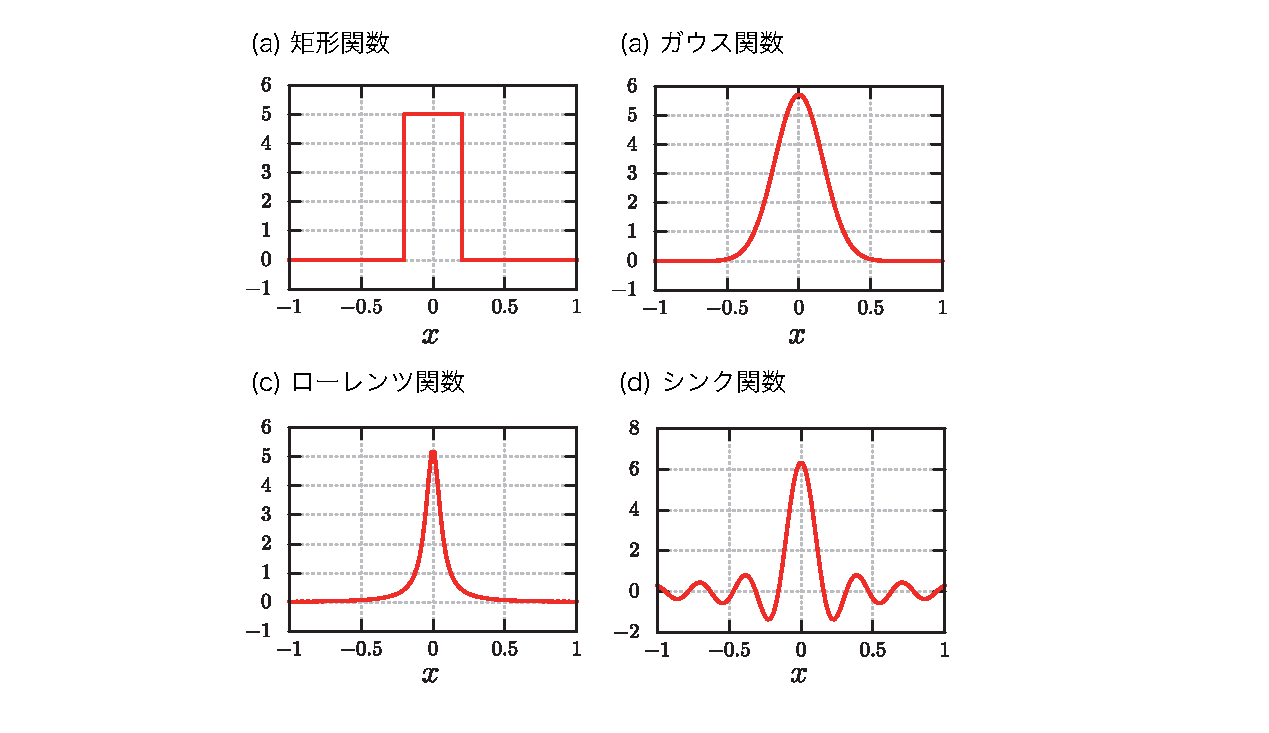
\includegraphics[width=1.0\linewidth]{/Users/kasa/Dropbox/GitHub/lectures/osaka-u/2021/kaenI/chap02_fr/figures/delta-func_explicit.eps} 
\end{figure}
%
\subsection{3次元空間のデルタ関数}
%
3次元空間
${\bf r} = (x,y,z)^{T}$ ($T$は転置を表す)
に対するデルタ関数$\delta\left({\bf r}\right)$は,
\begin{align}
 \delta\left({\bf r}\right) = \delta\left(x\right) \delta\left(y\right) \delta\left(z\right), 
\end{align}
で定義される.
%
%
\section{フーリエ変換}
%
再度,フーリエ積分の式\Eq{fourier_integral}を示しておく(ただし,変数$u$を$k$に変えている).
\begin{align}
 f\left(x\right) = \dfrac{1}{2\pi}\int_{-\infty}^{\infty}dk\,
                    \underline{\left(\int_{-\infty}^{\infty}dx^{\prime}\,f\left(x^{\prime}\right)e^{-ikx^{\prime}}\right)}e^{ikx}. \label{fourier_integral_02}
\end{align}
下線部は,フーリエ級数における展開係数$c_n$に対応するものであり,
これは関数$f(x)$に含まれる成分$k$\footnote{ここでは単に成分$k$と読んでいるが,$k$の呼び方は$x$が持つ次元によって名前が異なる.例えば,$x$が長さの次元を持つ場合,$k$を角波数とよび,$x$が時間の次元を持つときには角周波数(角振動数)と呼ぶ.多くの物理の教科書では,角波数と角周波数を$k$と$\omega$で使い分けている.}の波の量を表している.
そこで,$f(x)$から成分$k$の波の量を抽出する操作$\mathcal{F}[f(x)]$をフーリエ変換と呼び,変換後の関数を$F(k)$と表すことにすると,
\begin{align}
 F\left(k\right) = \mathcal{F}\left[f\left(x\right)\right] = \int_{-\infty}^{\infty}dx\, f\left(x\right)e^{-ikx},
\end{align}
である.また,変換して得られた関数$F\left(k\right)$のこと自体をフーリエ変換と呼ぶことがほとんどなので,混乱しないように.
$F\left(k\right)$から元々の関数$f\left(x\right)$に戻す操作のことをフーリエ逆変換$\mathcal{F}^{-1}\left[F(k)\right]$
と呼び,\Eq{fourier_integral_02}から,
\begin{align}
 f\left(x\right) = \mathcal{F}^{-1}\left[F\left(k\right)\right]
 = \dfrac{1}{2\pi} \int_{-\infty}^{\infty}dk\, F\left(k\right)e^{ikx},
\end{align}
である.

このテキストでの$x$座標のことを実空間,
$k$座標のことをフーリエ空間と呼ぶことがしばしばある.
このテキストでも,その名前をこれから使っていくことにする.
%
\subsection{3次元空間でのフーリエ変換}
%
3次元空間${\bf r}$の関数$f\left({\bf r}\right)$のフーリエ変換$F\left({\bf k}\right)$は次式のように表される.
\begin{align}
 F\left({\bf k}\right) &= \int_{-\infty}^{\infty}dx\int_{-\infty}^{\infty}dy \int_{-\infty}^{\infty}dz
                         e^{-ik_x x}e^{-ik_y y}e^{-ik_z z} f\left({\bf r}\right) \notag \\
                       &= \int d{\bf r}e^{-i{\bf k}\cdot {\bf r}}f\left({\bf r}\right).
\end{align}
%
逆変換は次式である.
\begin{align}
 f({\bf r}) &= \dfrac{1}{\left(2\pi\right)^3} \int_{-\infty}^{\infty}dx\int_{-\infty}^{\infty}dy \int_{-\infty}^{\infty}dz
              e^{ik_x x}e^{ik_y y}e^{ik_z z} F\left({\bf k}\right) \notag \\
            &=  \dfrac{1}{\left(2\pi\right)^3} \int_{-\infty}^{\infty}d{\bf k}\,e^{-i{\bf k}\cdot {\bf r}} F\left({\bf k}\right).
\end{align}
%
\subsection{デルタ関数のフーリエ変換}
%
デルタ関数$\delta(x)$は,次のような性質をもつものであった.
\begin{align}
 \int_{-\infty}^{\infty}dx\,\delta\left(x-a\right)f\left(x\right) = f\left(a\right). 
\end{align}
%
デルタ関数をフーリエ変換すると,
\begin{align}
 \int_{-\infty}^{\infty}dx\,e^{-ikx}\delta\left(x-a\right) = e^{-ika},
\end{align}
となる.
%
$a=0$の場合は,
\begin{align}
 \int_{-\infty}^{\infty}dx\,e^{-ikx}\delta\left(x\right) = 1, 
\end{align}
である\footnote{余談だが,知り合いの先生の御子息(小学生)は,「デルタ関数のフーリエ変換は何だ?言ってみろ」と父親から聞かれて,「イチ!」と答えたらしい.そのお子さんにはいつか「$\delta(x-a)$のフーリエ変換は?」と聞いてみたいところだ.}.
%
なので,1のフーリエ逆変換を考えると,
\begin{align}
 \delta\left(x\right) = \dfrac{1}{2\pi}\int_{-\infty}^{\infty}dk\,e^{ikx}, \label{deltafunc_fourier} 
\end{align}
が得られる.
%
\subsection{フーリエ変換が持つ性質}
%
フーリエ変換が持つ重要な性質について,以下でまとめておく.
無条件で成り立つわけではない関係式もあるので,それは導出過程で述べていくことにする
\footnote{ただし,ここでの導出は数学的に粗い部分がある.例えば,途中で現れる式の
フーリエ変換可能性などについての議論はいくつかすっ飛ばしている.気になる人はフーリエ解析や応用数学の教科書を参照すると良い.
大体のものに載っているはずである.}.
以下では,$F\left(k\right) = \mathcal{F}\left[f\left(x\right)\right],~G\left(k\right) = \mathcal{F}\left[g\left(x\right)\right]$,また$a,~b$は定数とする.
\begin{itemize}
  \item 線形性 
	\begin{align}
	  \mathcal{F}\left[af\left(x\right) + bg\left(x\right)\right] = aF\left(k\right) + bG\left(k\right)
	\end{align}

  \item 移動性
	\begin{align}
	  \mathcal{F}\left[e^{iax}f\left(x\right)\right] = F\left(k-a\right) \\
	  \mathcal{F}\left[f\left(x-a\right)\right]      = e^{-iak}F\left(k\right)
	\end{align}
  \item 拡大性
	\begin{align}
	  \mathcal{F}\left[f\left(ax\right)\right] = \dfrac{1}{\left|a\right|}F\left(\dfrac{k}{a}\right). 
	\end{align}
  \item 導関数のフーリエ変換 
	\begin{align}
	  \mathcal{F}\left[\dfrac{d^n}{dx^n}f\left(x\right)\right] = \left(ik\right)^{n} F\left(k\right)
	\end{align}
  \item 積分のフーリエ変換
	\begin{align}
	  \mathcal{F}\left[\int_{-\infty}^{x} dt\, f\left(t\right)\right] = \dfrac{1}{ik}F\left(k\right).
	\end{align}
  \item 畳み込み積分のフーリエ変換
	\begin{align}
	  \mathcal{F}\left[\int_{-\infty}^{\infty}dy\,f\left(y\right)g\left(x-y\right)\right] = F\left(k\right)G\left(k\right), \label{fourier_convolution}
	\end{align}

\end{itemize}
%
\subsubsection{線形性}
フーリエ変換では次の関係が成り立つ.
\begin{align}
 \mathcal{F}\left[af\left(x\right) + bg\left(x\right)\right] = aF\left(k\right) + bG\left(k\right).
\end{align}
これが成り立つのは,積分に線形性があるからである.つまり,
\begin{align}
 \mathcal{F}\left[af(x) + b g(x)\right] 
   &= \int_{-\infty}^{\infty}dx\,\left(af(x)+bg(x)\right)e^{-ikx} \notag \\
   &= a\int_{-\infty}^{\infty}dx\,f(x)e^{-ikx} + b\int_{-\infty}^{\infty}dx\,g(x)e^{-ikx} \notag \\
   &= aF(k) + bG(k).
\end{align}
%
%
\subsubsection{移動性}
%
$a$を定数として,次式が成り立つ.
%
\begin{align}
 \mathcal{F}\left[e^{iax}f\left(x\right)\right] = F\left(k-a\right), \\
 \mathcal{F}\left[f\left(x-a\right)\right]      = e^{-iak}F\left(k\right). 
\end{align}
%
1つ目は次のようにして示せる.
\begin{align}
 \mathcal{F}\left[e^{iax}f\left(x\right)\right] 
 &=\int_{-\infty}^{\infty}dx\,e^{iax}f\left(x\right)e^{-ikx} \notag \\
 &=\int_{-\infty}^{\infty}dx\,f\left(x\right)e^{-i\left(k-a\right)x} \notag \\
 &=F\left(k-a\right). 
\end{align}
2つ目は$X=x-a$と変数変換することで示せる.
\begin{align}
 \mathcal{F}\left[f\left(x-a\right)\right]      
 &= \int_{-\infty}^{\infty}dx\,f\left(x-a\right)e^{-ikx} \notag \\
 &= \int_{-\infty}^{\infty}dX\,f\left(X\right)e^{-ikx-ika} \notag \\
 &= e^{-ika}F\left(k\right).
\end{align}
%
\subsubsection{拡大性}
%
$a$を定数として,次に示す関係式が成り立つ.
\begin{align}
 \mathcal{F}\left[f\left(ax\right)\right] = \dfrac{1}{\left|a\right|}F\left(\dfrac{k}{a}\right). 
\end{align}
%
$X=ax$と変数変換を行うと,$a>0$のとき,
\begin{align}
 \int_{-\infty}^{\infty}dx\,e^{-ikx}f\left(ax\right) 
 & = \dfrac{1}{a} \int_{-\infty}^{\infty}dx\,f\left(X\right)e^{-i(k/a)X} \notag \\
 & = \dfrac{1}{a}F\left(\dfrac{k}{a}\right),
\end{align}
であり,$a<0$のとき
\begin{align}
 \int_{-\infty}^{\infty}dx\,e^{-ikx}f\left(ax\right) 
 & = \dfrac{1}{a} \int_{\infty}^{-\infty}dx\,f\left(X\right)e^{-i(k/a)X} \notag \\
 & = -\dfrac{1}{a}F\left(\dfrac{k}{a}\right),
\end{align}
従って,両方の場合を考慮すると,目的の式を得る.
%
\subsubsection{導関数のフーリエ変換}
%
$f(x)$の導関数のフーリエ変換は次式のように表すことができる.
\begin{align}
  \mathcal{F}\left[\dfrac{d^n}{dx^n}f\left(x\right)\right] = \left(ik\right)^{n} F\left(k\right). \label{deriv_fourier} 
\end{align}
無条件で成り立つわけではないが,それは導出の過程で述べることにする.
ここでは,1階の導関数の場合
\begin{align}
 \mathcal{F}\left[\dfrac{d}{dx}f\left(x\right)\right] = ik F\left(k\right),
\end{align}
の関係式を示しておくことにする.積の微分法より,
%
\begin{align}
 \mathcal{F}\left[\dfrac{d}{dx}f\left(x\right)\right] 
 &= \int_{-\infty}^{\infty}dx\,\dfrac{d}{dx}f\left(x\right)e^{-ikx} \notag \\
 &= \biggl[f\left(x\right)e^{-ikx}\biggr]_{-\infty}^{\infty} - \int_{-\infty}^{\infty}dx\,f\left(x\right)\dfrac{d}{dx}e^{-ikx} \notag \\ 
 &= \biggl[f\left(x\right)e^{-ikx}\biggr]_{-\infty}^{\infty} + ik \int_{-\infty}^{\infty}dx\,f\left(x\right)e^{-ikx} \notag \\
 &= \biggl[f\left(x\right)e^{-ikx}\biggr]_{-\infty}^{\infty} + ik F(k), 
\end{align}
となる.ここで,$\displaystyle\lim_{x\to \pm \infty}f\left(x\right)=0$という条件を課して,第1項をゼロにすると,目的の式が得られる.\footnote{正確に言うと,$f^{\prime}(x)$がフーリエ変換可能の場合($f^{\prime}(x)$が区分的になめらかで絶対可積分),$\displaystyle\lim_{x\to \pm}f(x) = 0$が成り立つので,目的の式が得られる.}.
$n$階の導関数の場合も全く同じ手続きで導出できる.

導関数が,フーリエ空間上では$F(k)$に$ik$をかけたものに変わるという性質は,
微分方程式を解く上で極めて有効である.
%
\subsubsection{フーリエ変換の微分}
%

フーリエ変換$F(k)$の微分について,次式が成り立つ.
\begin{align}
 \mathcal{F}\left[\left(-ix\right)^{n}f\left(x\right)\right] = \dfrac{d^n}{dk^n}F\left(k\right). 
\end{align}
%
$n=1$の場合を示しておく.
\begin{align}
  \dfrac{d}{dk}F\left(k\right)
  &= \dfrac{d}{dk}\int_{-\infty}^{\infty}dx\,f\left(x\right)e^{-ikx} \notag \\
  &= \int_{-\infty}^{\infty}dx\, \left(-ix\right)f\left(x\right)e^{-ikx} \notag \\
  &= \mathcal{F}\left[-ixf\left(x\right)\right].
\end{align}
$n=2$以降も同様にして示すことが出来る.
%
\subsubsection{積分のフーリエ変換}
%
$\int_{-\infty}^{\infty}dx\,f\left(x\right) = 0$を満たす関数$f(x)$について,次式が成り立つ.
%
\begin{align}
 \mathcal{F}\left[\int_{-\infty}^{x} dt\, f\left(t\right)\right] = \dfrac{1}{ik}F\left(k\right).
\end{align}
%
先ほどと同様,積の微分法から導くことが出来る.
\begin{align}
 \mathcal{F}\left[\int_{-\infty}^{x}dt\,f\left(t\right)\right] 
& = \int_{-\infty}^{\infty}dx\,\left(\int_{-\infty}^{\infty}dt\,f\left(t\right)\right) e^{-ikx} \notag \\
& = \left[\left(\int_{-\infty}^{x}dt\,f\left(t\right)\right)\dfrac{e^{-ikx}}{-ik}\right]_{-\infty}^{\infty}
    + \dfrac{1}{ik}\int_{-\infty}^{\infty}dx\, f\left(x\right)e^{-ikx} \notag \\
& = \dfrac{1}{ik}F\left(k\right). 
\end{align}
2行目の1項目が消えるのは,$\int_{-\infty}^{\infty}dx\,f\left(x\right) = 0$を仮定しているためである.
%
\subsubsection{畳み込み積分のフーリエ変換}
%
次式のような形で表される積分を畳み込み積分または合成積と呼ぶ.
\begin{align}
 I\left(x\right) = \int_{-\infty}^{\infty}dy\,f\left(y\right)g\left(x-y\right). 
\end{align}
また,上式は
\begin{align}
 I\left(x\right) = \int_{-\infty}^{\infty}dy\,f\left(x-y\right)g\left(y\right),
\end{align}
と等価である(変数変換を試してみればすぐ分かる).
%
理学・工学問わず現れる重要な形の積分である.
\footnote{例えば,私が専門とする液体論では,$h({\bf r}) = c\left({\bf r}\right) + \rho \int d{\bf r}^{\prime}\,c\left({\bf r}^{\prime}\right)h\left({\bf r}-{\bf r}^{\prime}\right)$という形の方程式が,液体の微視的状態を記述する上で重要となる.この式にも畳み込み積分が含まれている.}
%
畳み込み積分をフーリエ変換すると,
%
\begin{align}
 \mathcal{F}\left[\int_{-\infty}^{\infty}dy\,f\left(y\right)g\left(x-y\right)\right] = F\left(k\right)G\left(k\right),
\end{align}
%
のように表される.
この式は,畳み込み積分を計算したかったら,$f(x)$と$g(x)$をそれぞれフーリエ変換して,それらの積をとれば良い,
ということを主張するものであり,理論的な式変形だけでなく数値解析上も極めて有用なものである.
一方で,その導出はシンプルである.まず,
\begin{align}
 e^{-ikx} = e^{-ik\left(x-y\right)}e^{-iky}, 
\end{align}
%
と書き換えることを考える.つまり,
%
\begin{align}
 \mathcal{F}\left[I\left(x\right)\right]
 &= \int_{-\infty}^{\infty}dx\,e^{-ikx}\int_{-\infty}^{\infty}dy\,f\left(y\right)g\left(x-y\right) \notag \\
 &= \int_{-\infty}^{\infty}dy\,\left(f\left(y\right)e^{-iky} \underline{\int_{-\infty}^{\infty}dx\,g\left(x-y\right)e^{-ik\left(x-y\right)}}\right),
\end{align}
%
のようにする.下線部は$G\left(k\right)$なので,
\begin{align}
 \mathcal{F}\left[I\left(x\right)\right] 
 &= \int_{-\infty}^{\infty}dy\,f\left(y\right)e^{-iky}G\left(k\right)\notag \\
 &= F\left(k\right)G\left(k\right),
\end{align}
とできて,目的の式を得る.
%
%
\subsubsection{積のフーリエ変換}
%
今度は積$f(x)g(x)$のフーリエ変換を考えてみよう.実は,実空間での関数の積はフーリエ空間上では
畳み込み積分になる.
%
\begin{align}
 \mathcal{F}\left[f\left(x\right)g\left(x\right)\right] = \dfrac{1}{2\pi}\int_{-\infty}^{\infty}dk\, 
              F\left(k^{\prime}\right) G\left(k-k^{\prime}\right). 
\end{align}
つまり,フーリエ変換することで式変形が厄介になる.

この式を導出するには,まず$f(x)$と$g(x)$のどちらかをフーリエ逆変換の形で表しておく.
\begin{align}
  \mathcal{F}\left[f\left(x\right)g\left(x\right)\right]
  &= \int_{-\infty}^{\infty}dx\,e^{-ikx}\left(\dfrac{1}{2\pi}\int_{-\infty}^{\infty}dk^{\prime}\,e^{ik^{\prime}x}F\left(k\right)\right)g\left(x\right). 
\end{align}
次に,$e^{-ikx}e^{ik^{\prime}x} = e^{-i(k-k^{\prime})x}$のように,ひとまとめにすることで,
\begin{align}
  \mathcal{F}\left[f\left(x\right)g\left(x\right)\right]
  &= \dfrac{1}{2\pi}\int_{-\infty}^{\infty}dk^{\prime}\,\left(F\left(k^{\prime}\right)\int_{-\infty}^{\infty}dx\,e^{-i(k-k^\prime)x}g\left(x\right)\right) \notag \\
  &= \dfrac{1}{2\pi}\int_{-\infty}^{\infty}dk^{\prime}\,F\left(k^{\prime}\right)G\left(k-k^{\prime}\right),
\end{align}
を得る.
%
\newpage
\hrule
\reidai
ガウス関数
\begin{align}
  f\left(x\right) = e^{-ax^2}, \quad (a>0)
\end{align}
のフーリエ変換を求めよ.
\vspace*{.2cm}
\hrule
\vspace*{.2cm}
%
$f(x)$のフーリエ変換を$F(k)$とおくと,
\begin{align}
 F(k) & = \int_{-\infty}^{\infty}dx\, e^{-ikx}e^{-ax^2},
\end{align}
である.まず,指数部分は,
\begin{align}
 -ikx - ax^2 = -a\left(x+\dfrac{ik}{2a}\right)^2 -\dfrac{k^2}{4a}, 
\end{align}
のように平方完成出来るので,
\begin{align}
  F\left(k\right)
  &= \int_{-\infty}^{\infty}dx\,\exp\left[-a\left(x+\dfrac{ik}{2a}\right)^2-\dfrac{k^2}{4a}\right] \notag \\
  &= \exp\left(-\dfrac{k^2}{4a}\right) \int_{-\infty}^{\infty}dx\,\exp\left[-a\left(x+\dfrac{ik}{2a}\right)^2\right], 
\end{align}
となる.ガウス積分\footnote{ガウス積分について未習の場合は,公式として受け入れてほしい.心配しなくても,必ず量子力学の講義で学ぶことになる.}
\begin{align}
 \int_{-\infty}^{\infty}dx\,e^{-ax^2} = \sqrt{\dfrac{\pi}{a}}, 
\end{align}
を用いることで,
\begin{align}
  F\left(k\right) = \sqrt{\dfrac{\pi}{a}}\exp\left(-\dfrac{k^2}{4a}\right), 
\end{align}
を得る\footnote{実はこの解法には少しごまかしが入っているが,その点を理解するためには複素関数論の知識が必要となるので,今回はこれで良しとする.もちろん,結果は正しい.}.
%
\newpage
\hrule
\reidai
次の$f(x)$に関する方程式を解け.
\begin{align}
  \int_{-\infty}^{\infty}dy\,f(y)f(x-y) = \sqrt{\dfrac{a}{\pi}}e^{-ax^2} \quad (a>0) 
\end{align}
\hrule
\vspace*{.2cm}

両辺をフーリエ変換すると,
\begin{align}
  \left(F\left(k\right)\right)^2 = e^{-k^2/4a}.
\end{align}
よって,
\begin{align}
  F\left(k\right) = \pm e^{-k^2/8a},
\end{align}
なので,逆変換すると,
\begin{align}
 f\left(x\right) &= \pm \dfrac{1}{2\pi}\int_{-\infty}^{\infty}dk\,e^{ikx}e^{-k^2/8a} \notag \\
                 &= \sqrt{\dfrac{2a}{\pi}}\exp(-2ax^2). 
\end{align}
